\documentclass[twocolumn,showpacs,unsortedaddress,superscriptaddress,showkeys,nofootinbib,preprintnumbers,letterpaper]{revtex4-1}
\usepackage{acronym}
\usepackage{amsmath}
\usepackage{amssymb}
\usepackage{graphics}
\usepackage{subfigure}
\usepackage[squaren]{SIunits}
\usepackage[usenames]{color}

\newcommand{\FIXME}[1]{\textcolor{red}{\textbf{#1}}}

\newcommand*{\ee}{\mathrm{e}}
\newcommand*{\aye}{\mathrm{i}}
\newcommand*{\diff}{\,\mathrm{d}}
\newcommand{\abs}[1]{\left\lvert #1 \right\rvert}
\newcommand{\chisq}{\chi^{2}}
\newcommand{\Deff}{D_{\mathrm{eff}}}
\newcommand{\Dh}{{D_{\mathrm{H}}}}
\newcommand{\Dnl}{\tilde{D}}
\newcommand{\figref}[1]{FIG.\ \ref{#1}}
\newcommand{\lr}{\mathcal{L}}
\newcommand{\mean}[1]{\left\langle#1\right\rangle}
\newcommand{\Msun}{M_{\odot}}
\newcommand{\noise}{\mathrm{noise}}
\newcommand{\norm}[1]{\left\lVert #1 \right\rVert}
\newcommand{\signal}{\mathrm{signal}}
\newcommand{\sigparams}{\bar{\theta}}
\newcommand{\snr}{\rho}
\newcommand{\ptjtk}{\rho(\vec{t}_j\cdot\vec{t}_k)}     
\newcommand{\tjtk}{(\vec{t}_j\cdot\vec{t}_k)}    
\newcommand{\tjtkk}{(\vec{t}_j\cdot\vec{t}_{k'})}    
\newcommand{\ptjtkk}{\rho(\vec{t}_j\cdot\vec{t}_{k'})}  
\newcommand{\rhok}{\rho_{\text{obs,$k$}}}  


\addunit{\annum}{a}
\addunit{\parsec}{pc}

\DeclareMathOperator{\order}{O}

\begin{document}


%%%%%%%%%%%%%%%%%%%%%%%%%%%%%%%%%%%%%%%%%%%%%%%%%%%%%%%%%%%%%%%%%%%%%%%%%%%%%%%
% TITLE, AUTHOR
%%%%%%%%%%%%%%%%%%%%%%%%%%%%%%%%%%%%%%%%%%%%%%%%%%%%%%%%%%%%%%%%%%%%%%%%%%%%%%%

\title{Source-dependent likelihood-ratio detection statistic for compact binary coalescence candidates}

\author{Heather Fong}
\email{heather.fong@ligo.org}
\affiliation{Canadian Institute for Theoretical Astrophysics, University of Toronto, Toronto, ON, M5S 3H8, Canada}
\affiliation{Department of Physics, University of Toronto, Toronto, ON, M5S 3H8, Canada}

\author{Kipp Cannon}
\email{kipp.cannon@ligo.org}
\affiliation{RESCEU, University of Tokyo, Tokyo, 113-0033, Japan}

\author{Other authors}
\email{authors@email.com}
\affiliation{School info}

\begin{abstract}
Abstract goes here.
\end{abstract}

% 02. 	Mathematical methods in physics
% 02.50.-r 	Probability theory, stochastic processes, and statistics
%	02.50.Ey 	Stochastic processes
%	02.50.Sk 	Multivariate analysis
%	02.50.Tt 	Inference methods
% 02.70.-c 	Computational techniques; simulations
%	02.70.Uu 	Applications of Monte Carlo methods
%
% 04. 	General relativity and gravitation
% 04.30.-w 	Gravitational waves
%	04.30.Tv 	Gravitational-wave astrophysics
%
% 07. 	Instruments, apparatus, and components common to several branches of physics and astronomy
% 07.05.-t 	Computers in experimental physics
%	07.05.Kf 	Data analysis: algorithms and implementation; data management
%
% 95. 	Fundamental astronomy and astrophysics; instrumentation, techniques, and astronomical observations
% 95.75.-z 	Observation and data reduction techniques; computer modeling and simulation
%	95.75.Pq 	Mathematical procedures and computer techniques
%
% 97. 	Stars
% 97.80.-d 	Binary and multiple stars

\pacs{02.50.Ey, 02.50.Sk, 02.50.Tt, 02.70.Uu, 04.30.Tv, 07.05.Kf, 95.75.Pq, 97.80.-d}

\maketitle
%\input{acros}

%%%%%%%%%%%%%%%%%%%%%%

\FIXME{Comments for Kipp (Hi, Kipp!):
\begin{itemize}
\item{Should we change 'ranking statistic' to 'detection statistic' to match the CBC paper?}
\item{I can't get bibtex to work for some reason, so suggestions of citations are labelled in red (I get a 'Warning--jnrlst (dependency: not reversed) set 1
merlin.mbs apsrev4-1.bst 2010-07-25 4.21a (PWD, AO, DPC) hacked' warning when I run bibtex).}
\item{What BBH probability distribution function should we use, so we can show both BNS and BBH results of the template weighting?}
\item{I gave a stab at describing $P(\vec\theta|\text{noise})$ (below Equation \ref{eqn:L_theta}), but I think I've said incorrect things.}
\end{itemize}}

\section{Introduction}

The direct detections of gravitational waves by the Advanced Laser Interferometer Gravitational-wave Observatory (Advanced LIGO) that were made in late 2015 \FIXME{[GW150914, GW151226, O1 papers]} have propelled us into the age of gravitational-wave astronomy. Additional gravitational-wave observatories are also expected to come online in in the next several years. With further observation runs scheduled and additional improvements planned for the current LIGO detectors, the rate at which gravitational waves from compact binary coalescences are observed is expected to increase \FIXME{[rates paper]}. With additional detections occurring more and more frequently, we stand to gain a deeper understanding of these tumultuous and dramatic astrophysical events. 

Searches for gravitational waves from compact binary coalescences use a technique known as matched-filtering, which involves correlating the detector data with template waveforms. The template waveforms comprise a template bank, and model the expected signal of gravitational waves from binary neutron stars, binary black holes, and neutron star-black hole binaries. Candidate events are identified through matched-filtering, and they are assigned a detection statistic that assesses their likelihood of being a gravitational-wave signal. 

In \FIXME{Cannon \textit{et al}} derives a likelihood-ratio detection statistic that expands on previous work by \FIXME{Biwas \textit{et al.}} and \FIXME{Aasi \textit{et al.}} and incorporates a model for the correlations in the signal-to-noise-ratios with which signals will be seen in a network of ground-based antennae. The detection statistic retains an algebraic procedure for mapping detection statistic values to false-alarm probability. The detection statistic derived by Cannon \text{et al.} has been implemented into one of Advanced LIGO's compact binary coalescence gravitational-wave searches.

Currently, this likelihood ratio-based detection statistic carries the assumption that gravitational-wave signals are equally likely to be recovered by any waveform template in the template bank. This assumption has been implicitly chosen in past gravitational-wave searches from compact binary coalescences, but carries no astrophysical information from source population models. As a result, compact binary coalescence searches suffer in sensitivity because it assumes an incorrect distribution of compact binaries in the Universe. 

This article presents a derivation that folds in astrophysical source population model information into the detection statistic. It will also tune compact binary coalescence searches to be more sensitive to a given population, which will improve the accuracy of the rate estimates of observed mergers. 

In Section \ref{sec:rankingstat}, we begin by describing the detection statistic that is currently used in Advanced LIGO's low-latency searches for compact binary coalescences. The derivation of a ranking statistic that envelops astrophysical source model information is outlined in Section \ref{sec:derivation}, where the various terms are explored in further detail in Sections \ref{sec:}, \ref{sec:}, and \ref{sec:}. Finally, in Section \ref{sec:}, we present a discussion of the new detection statistic, and conclude in Section \ref{sec:}.

%%%%%%%%%%%%%%%%%%%%%%%%%%
%%%%%%%%%%%%%%%%%%%%%%%%%%

\section{Likelihood-ratio detection statistic} \label{sec:rankingstat}

The detection statistic employed in one of Advanced LIGO's compact binary coalescence searches is the likelihood ratio, which is an effective way to rank signals because of the known mapping between the detection statistic value and false-alarm probability. The likelihood-ratio detection statistic is given as the following (adapted from Eq. 1 of \FIXME{[arXiv:1504.04632]}):
	\begin{widetext}
	\begin{multline}
	\label{eqn:LR}
	\mathcal{L}(\{D_{H_{H1}}, D_{H_{L1}}, ...\}, \{H1, L1, ...\}, \rho_{H1}, \chi^2_{H1}, \rho_{L1}, \chi^2_{L1}, ..., \vec{\theta}) \\
	= \mathcal{L}(...| \vec{\theta}) \mathcal{L}(\vec{\theta}) = \frac{P(\{D_{H_{H1}}, D_{H_{L1}}, ...\}, \{H1, L1, ...\}, \rho_{H1}, \chi^2_{H1}, \rho_{L1}, \chi^2_{L1}, ... | \vec{\theta}, \text{signal})}{P(\{D_{H_{H1}}, D_{H_{L1}}, ...\}, \{H1, L1, ...\}, \rho_{H1}, \chi^2_{H1}, \rho_{L1}, \chi^2_{L1}, ... | \vec{\theta}, \text{noise})} \mathcal{L}(\vec{\theta}), 
	\end{multline}
	\end{widetext}
where $\{D_{H_{H1}}, D_{H_{L1}}, ...\}$ is the set of horizon distances for all instruments in the network at the time of the observed event, $\{H1, L1, ...\}$ is the set of instruments that observed the event, $\rho$ and $\chi^2$ are the template matched-filter signal-to-noise ratios (SNRs) and $\chi^2$ values for the candidate in those instruments, and $\vec{\theta}$ are the intrinsic parameters of the template. The first term in Eq. \ref{eqn:LR} is worked out in detail in \FIXME{[arXiv:1504.04632]}.

The second term in the equation, $\mathcal{L}(\vec{\theta})$, is also a fraction:
	\begin{equation}
	\mathcal{L}(\vec{\theta}) = \frac{P(\vec{\theta}|\text{signal})}{P(\vec{\theta}|\text{noise})}.
	\label{eqn:L_theta}
	\end{equation}
\FIXME{The denominator, $P(\vec{\theta}|\text{noise})$, is the probability of recovering a template waveform with parameters $\vec{\theta}$ given that there is no signal in the data. The mean rate for a template waveform of detector is measured by counting the number of triggers collected over some large interval of time. Coincidences are computed by determining whether triggers are found within the coincident time window of the different detectors, and this information is used to calculate the mean rate of coincidences. $P(\vec{\theta}|\text{noise})$ is then obtained by dividing that rate by the sum of all those rates for all $\vec\theta$.} 
$P(\vec{\theta}|\text{signal})$ is the probability that a template waveform with parameters $\vec{\theta}$ is recovered as the best-match template waveform, given that there is a signal in the data. Currently, $P(\vec{\theta}|\text{signal})$ is chosen to be uniform in the waveform space comprising the template bank, such that all templates are equally likely in the signal population. However, because the spacing between template waveforms is determined by the noise spectrum of the detectors rather than the physical properties of the sources, this prior does not contain astrophysically meaningful quantities. 

In the following sections, we derive a new expression for $P(\vec{\theta}|\text{signal})$ such that it incorporates astrophysical priors into the template weighting. This calculation allows us to then develop a likelihood-ratio detection statistic that incorporates our choice of astrophysical source population model. 

%%%%%%%%%%%%%%%%%%%%%%%%%%
%%%%%%%%%%%%%%%%%%%%%%%%%%

\section{Derivation} \label{sec:derivation}

We consider a gravitational-wave candidate $\vec{s}$; it belongs to an astrophysical source population $\mathcal{S}$ and has parameters $\vec\theta$:
   \begin{equation}
   \vec\theta = \{m_1,m_2,\chi,\rho\},
   \label{eqn:theta}
   \end{equation}
where $m_1$ and $m_2$ are the source masses, $\chi$ is the effective spin, and $\rho$ is the nominal signal-to-noise ratio (SNR). 

We assume that the waveform template bank is densely populated such that the candidate can be described by a template $\vec{t}_j$ in the bank multiplied by some SNR $\rho$. Therefore, the candidate is expressed as $\vec{s}(\vec\theta)=\rho\vec{t}_j(\vec\theta)$. The candidate also contains noise $\vec{n}$, which is assumed to be stationary Gaussian noise. To simplify the notation, the dependency on $\vec{\theta}$ is implied from this point on. 

Given that there is a candidate that is known to look like $\vec{s}=\rho\vec{t}_j$, the probability that a signal from a specified source population is recovered by a template $\vec{t}_k$ is
   \begin{multline}
   \label{eqn:prob_signal}
   P(\vec{t}_k | \text{signal})\\
   = \sum_j \Big\{ P(\vec{t}_j|\text{signal})\times P(\text{candidate in }\vec{t}_k|\vec{s}=\rho\vec{t}_j) \Big\},
   \end{multline}
where $P(\text{candidate in }\vec{t}_k|\vec{s}=\rho\vec{t}_j)$ is the probability that template $\vec{t}_k$ is the best match for the candidate. $\vec{t}_k$ is the $k$th template that lies on the unit sphere in waveform space (as shown in Figure \ref{fig:unitsphere}); therefore, $|\vec{t}_k| = 1$. $P(\vec{t}_j|\text{signal})$ is the probability that a signal is described by a template on the unit sphere, and it is given by an astrophysical source model.
	\begin{figure}
	\resizebox{0.7\linewidth}{!}{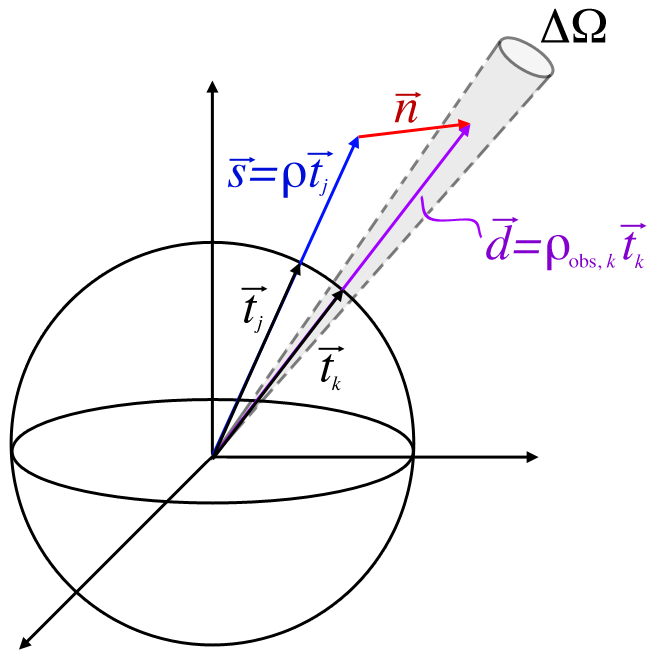
\includegraphics{unitsphere.png}}
	\caption{Unit sphere.}
	\label{fig:unitsphere}
	\end{figure}
From here, we can see there are two parts to this derivation: there is $P(\vec{t}_j|\text{signal})$, which depends only on the source population, and there is $P(\text{candidate in }\vec{t}_k|\vec{s}=\rho\vec{t}_j)$, which depends on the signal and the template bank. We will begin with deriving the former.

%%%%%%%%%%%%%%%%%%%%%%%%%%
%%%%%%%%%%%%%%%%%%%%%%%%%%

\section{$P(\vec{t}_j|\text{signal})$}

The first term in the summation of Eq. \ref{eqn:prob_signal} depends on the astrophysical source population model; therefore, a choice must be made for the source population model. In this work, we will consider two models: a binary neutron star (BNS) population and a binary black hole (BBH) population.

The probability density function (PDF) of the source population is given as $P(\vec{\gamma})$, where $\vec{\gamma}=\{\gamma_1,\gamma_2,..., \gamma_M\}$ are the intrinsic parameters of the source population, such as the masses and spins. The probability of that a signal looks like $\vec{t}_j$ (multiplied by some $\rho$) is the following:
	\begin{align}
	P(\vec{t}_j|\text{signal}) &= \int P_j(\vec{\gamma}) \diff\vec{\gamma} \\
	&\approx P_j(\gamma_1) P_j(\gamma_2)...P_j(\gamma_M) \times V_j.
	\end{align}
In the final equality, we assume that the distribution of the source parameters are independent of one another, so the joint probability is the product of the marginals. $V_j$ is the $M$-dimensional volume of the $j$th region of the Voronoi diagram, and it is assumed that $V_j$ is small enough such that $P_j(\gamma_i)$ is constant along in the patch. We compute this for each template in the template bank to find the probability that a system from the given source population will have the same properties as the template. 

The BNS source population we used is from \FIXME{[arXiv: 1309.6635]}, and the results are summarized in Figure~\ref{fig:P_BNS}. We use the BBH source population from \FIXME{[BBH PDF source]}, and the results are summarized in Figure~\ref{fig:P_BBH}.

	\begin{figure}
	\resizebox{\linewidth}{!}{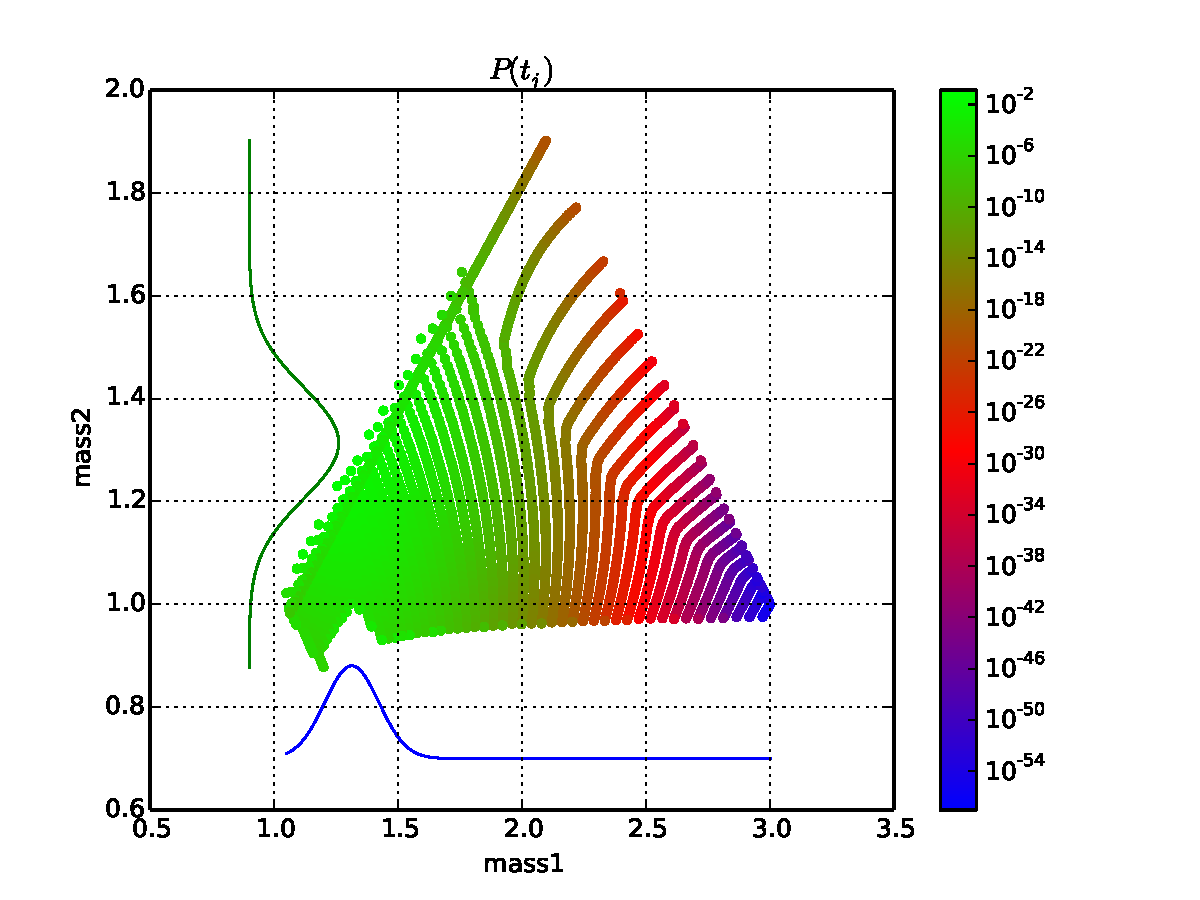
\includegraphics{first2years_20160612_Pj_100templates_N3.pdf}}
	\caption{$P(\vec{t}_j|\text{signal})$ calculated for each template in the bank. Plotted on the figure in solid lines are the mass probability distributions from which the source population follows. Some templates are not included because their calculated areas are far too large, due to the computed Voronoi regions. \FIXME{Placeholder plot.}}
	\label{fig:P_BNS}
	\end{figure}

%%%%%%%%%%%%%%%%%%%%%%%%%%
%%%%%%%%%%%%%%%%%%%%%%%%%%

\section{$P(\text{candidate in }\vec{t}_k|\vec{s}=\rho\vec{t}_j)$}

When a candidate $\vec{s}$ is detected by the instruments, the resulting signal has an additional factor due to noise $\vec{n}$ that is assumed to be stationary and Gaussian-distributed. Therefore, the detected signal $\vec{d}$ is given as the sum of the candidate $\vec{s}$ and the noise $\vec{n}$. We assume that $\vec{d}$ can also be described by a waveform template, denoted as $\vec{t}_k$, multiplied by some observed SNR $\rhok$.

   \begin{align}
   \vec{d} &= \vec{n} + \vec{s} \\
   \rhok\vec{t}_k &= \vec{n} + \rho\vec{t}_j,
   \end{align}
where $\rhok$ is the observed SNR. Again, we assume that that signal $\vec{s}$ is described by a template $\vec{t}_j$ in the bank. We also assume that template $\vec{t}_k$ is the best-fitting template to the detected signal $\vec{d}$. $|\vec{n}|^2$ then becomes 
   \begin{align}
   |\vec{n}|^2 &= (\rhok\vec{t}_k - \rho\vec{t}_j) \cdot (\rhok\vec{t}_k - \rho\vec{t}_j)\\
               &= \rho^2 + \rhok^2 - 2\rhok\ptjtk
   \label{eqn:n_squaredmagnitude}
   \end{align}
Because $\vec{n}$ is assumed to follow a Gaussian distribution with a constant variance of 1, the probability density function for $N$ dimensions is given as
   \begin{equation}
   f(\vec{n}) = \frac{1}{(2\pi)^{N/2}}e^{-\frac{1}{2}|\vec{n}|^2}
   \end{equation}
We want to find the probability that $\vec{d}=\rho\vec{t}_j+\vec{n}$ lies inside the conic volume of some template $\vec{t}_k$ with solid angle $\Delta\Omega$, where $\Delta\Omega$ is determined by the density of the template bank; refer to Fig~\ref{fig:unitsphere}. If $\vec{d}$ is inside the conic volume, it means that it is recovered by that template $\vec{t}_k$.

The probability that any signal is recovered by $\vec{t}_k$ can then be expressed as a ratio of the probability density of one template over the sum of probability densities of all the templates in the bank:
   \begin{multline}
   \label{eqn:prob_s_recovered_by_tk}
   P(\text{candidate in }\vec{t}_k|\vec{s}=\rho\vec{t}_j) \\= \frac{\int_0^\infty \frac{1}{(2\pi)^{N/2}} e^{-\frac{1}{2} |\vec{n}|^2} {\rhok^{N-1}} \diff\rhok \Delta\Omega}
   {\sum_{\vec{t}_{k'}} \int_0^\infty \frac{1}{(2\pi)^{N/2}} e^{-\frac{1}{2} |\vec{n}|^2} {\rhok^{N-1}} \diff\rhok \Delta\Omega}
   \end{multline}

We deal with the numerator in Eq. \ref{eqn:prob_s_recovered_by_tk} first. Moving constant terms outside the integral and substituting $|\vec{n}|^2$ with Eq. \ref{eqn:n_squaredmagnitude}, we obtain
   \begin{equation}
   = \frac{\Delta\Omega}{(2\pi)^{N/2}} \int_0^\infty  e^{-\frac{1}{2}( \rho^2 + \rhok^2 - 2\rhok\ptjtk)  } {\rhok^{N-1}} \diff\rhok
   \label{eqn:P_k01}
   \end{equation}
   \begin{equation}
  = \frac{\Delta\Omega}{(2\pi)^{N/2}} e^{-\frac{1}{2}\rho^2(1-(\vec{t}_j\cdot\vec{t}_k)^2)} \int_0^\infty  e^{-\frac{1}{2} (\rhok - \ptjtk)^2  } {\rhok^{N-1}} \diff\rhok
  \label{eqn:P_k02}
   \end{equation}
For the exponential term, we use the completing the square technique in the first equality of Eq.~\ref{eqn:P_k01} to obtain Eq.~\ref{eqn:P_k02}. Letting $N\!=\!4$ (which is the number of dimensions in $\vec{\theta}$, see Eq. \ref{eqn:theta}), the integrand $I$ in Eq. \ref{eqn:P_k01} becomes
	\begin{multline}
	 I = \int_0^\infty  e^{-\frac{1}{2} (\rhok - \ptjtk)^2  } {\rhok^{3}} \diff\rhok\\
	 \hspace{1.5em}= \sqrt{\frac{\pi}{2}}\ptjtk\Big[(\ptjtk)^2+3\Big]\Big[1+\mathrm{erf}\Big(\frac{\ptjtk}{\sqrt{2}}\Big)\Big]+\\
	 e^{-\frac{1}{2}(\ptjtk)^2}\Big[(\ptjtk)^2+2\Big]
	 \end{multline}
Therefore, we obtain the following expression in the numerator:
	\begin{widetext}
	\begin{multline}
	\int_0^\infty \frac{1}{(2\pi)^{2}} e^{-\frac{1}{2} |\vec{n}|^2} {\rho^{3}_{obs,k}} d\rho_{obs,k} \Delta\Omega \\
	= \frac{\Delta\Omega}{(2\pi)^{2}} e^{-\frac{1}{2}\rho^2} e^{\frac{1}{2}(\ptjtk)^2}\Big\{ \sqrt{\frac{\pi}{2}}\Big[(\ptjtk)^3+3\ptjtk \Big]\Big[1+\mathrm{erf}\Big(\frac{\ptjtk}{\sqrt{2}}\Big)\Big]+e^{-\frac{1}{2}(\ptjtk)^2}\Big[(\ptjtk)^2+2\Big] \Big\}
	\end{multline}
	\end{widetext}
The denominator is calculated in the same way. When we compute the full probability from Eq.~\ref{eqn:prob_s_recovered_by_tk}, the factor $\frac{\Delta\Omega}{(2\pi)^{2}} e^{-\frac{1}{2}\rho^2}$ appears in both numerator and denominator, and thus, cancel out. Therefore, the final probability becomes the following:
	\begin{widetext}
	\begin{multline}
	P(\text{candidate in }\vec{t}_k|\vec{s}=\rho\vec{t}_j) =\\
	\frac{
	e^{\frac{1}{2}\rho^2\tjtk^2}
	\sqrt{\frac{\pi}{2}}\Big[(\ptjtk)^3+3\ptjtk \Big]\Big[1+\mathrm{erf}\Big(\frac{\ptjtk}{\sqrt{2}}\Big)\Big]+(\ptjtk)^2+2
	}{
	{\sum_{\vec{t}_{k'}} \Big\{e^{\frac{1}{2}\rho^2\tjtkk^2} \sqrt{\frac{\pi}{2}}\Big[(\ptjtkk)^3+3\ptjtkk\Big]\Big[1+\mathrm{erf}\Big(\frac{\ptjtkk}{\sqrt{2}}\Big)\Big]+(\ptjtkk)^2+2\Big\}
	}}
	\label{eqn:p_k}
	\end{multline}
	\end{widetext}

%%%%%%%%%%%%%%%%%%%%%%%%%%
%%%%%%%%%%%%%%%%%%%%%%%%%%

\section{$P(\vec{t}_k | \text{signal})$}

\FIXME{Results need to be updated}

Now that we have derived all components, we can calculate the probability that any signal in our source population is recoverable by a particular template; that is, $P(\vec{t}_k | \text{signal})$ from Eq.~\ref{eqn:prob_massbin}.

	\begin{figure}
	\resizebox{\linewidth}{!}{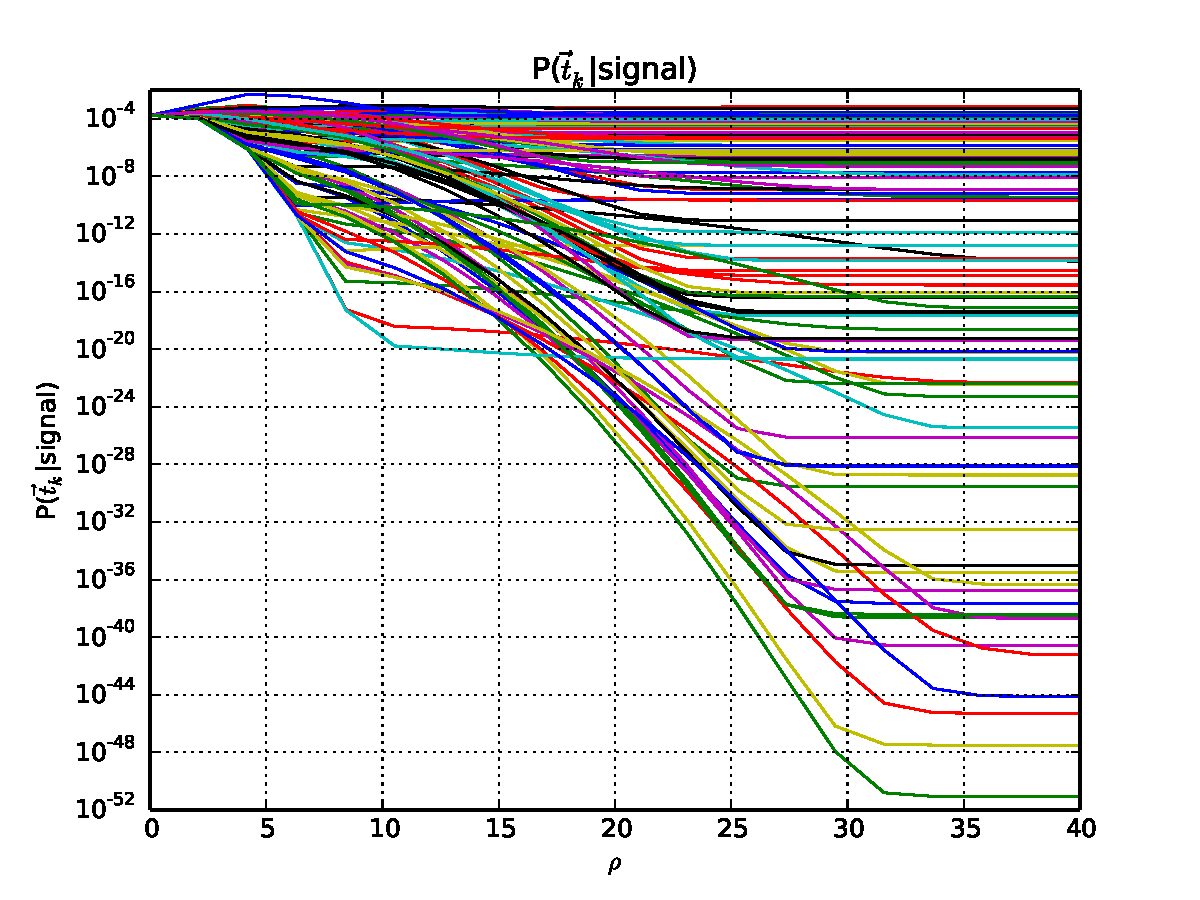
\includegraphics{first2years_20160612_Pvsrho_100templates_N3.pdf}}
	\resizebox{\linewidth}{!}{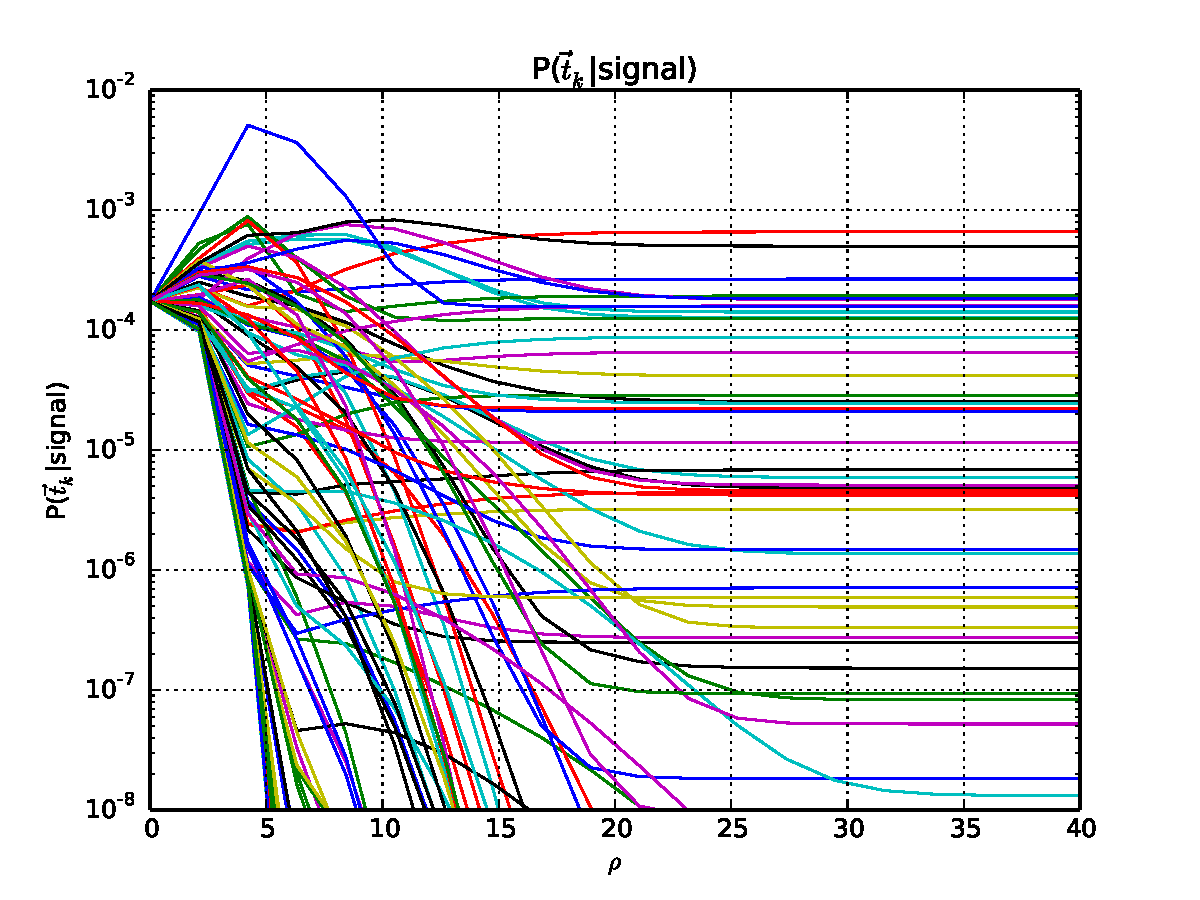
\includegraphics{first2years_20160612_Pvsrho_zoom_100templates_N3.pdf}}
	\caption{The probability $P$ as a function of $\rho$ for 100 templates in the ``first2years" template bank. Some templates have a local maximum at $10\lesssim \rho\lesssim 5$ before either asymptotically approaching a constant. The right panel is a zoomed-in version of the left panel.}
	\label{fig:Pvsrho}
	\end{figure}

In this study, we use the ``first2years" template bank, which consists of $\sim\!5700$ non-spinning templates. %The grey stars in the same figure represent the BNS source population, from which 1000 sources are drawn from the mass probability distribution given by \href{https://arxiv.org/abs/1309.6635}{Kiziltan {\it et al.}, 2013}. Following our assumption that $\vec{s}=\rho\vec{t}_j$, the sources are sampled directly from the template bank.
We randomly select 100 templates from the template bank to calculate $P(\text{all $\vec{s}$ in $\mathcal{S}$ is recoverable by $\vec{t}_k$})$. The probabilities are also calculated at different $\rho$ to observe how the recoverability of the templates change with stronger or weaker signals. We plot $P(\text{all $\vec{s}$ in $\mathcal{S}$ is recoverable by $\vec{t}_k$})$ vs. $\rho$ in Figure~\ref{fig:Pvsrho} for the 100 templates. Some of the curves have a local maximum at $10\lesssim \rho\lesssim 5$ before asymptotically approaching a constant, which indicates that low-SNR populations will appear to have a different mass distribution than high-SNR populations.

To better understand which templates give asymptotically approach a constant value with increasing $\rho$, in Figure~\ref{fig:P_tkj}, we show the templates mapped onto mass axes, with the colours denoting the magnitude of the calculated probability. As $\rho$ increases, we see that the probabilities of most templates exponentially decrease, except for a collection of templates that are clustered around the source population.
	\begin{figure}
	\resizebox{\linewidth}{!}{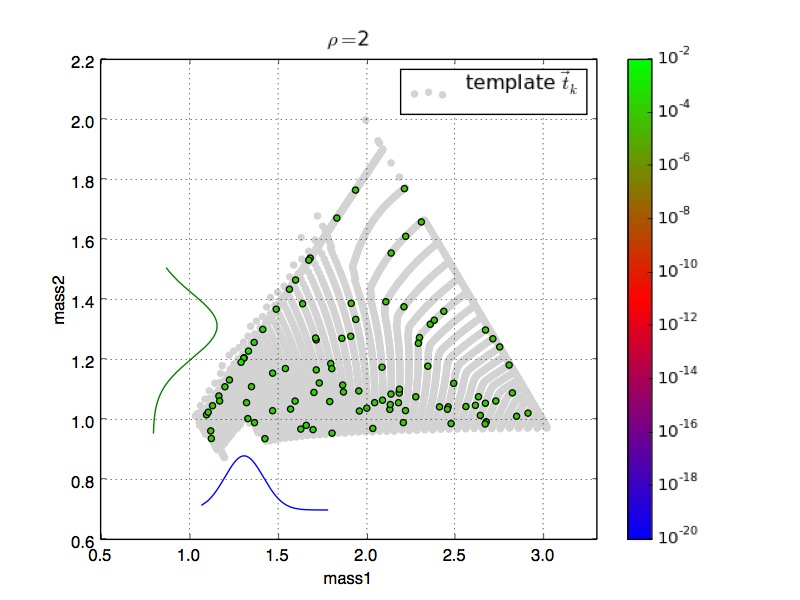
\includegraphics{first2years_20160612_P_tkj_100templates_2rho_N3.jpg}}
	\resizebox{\linewidth}{!}{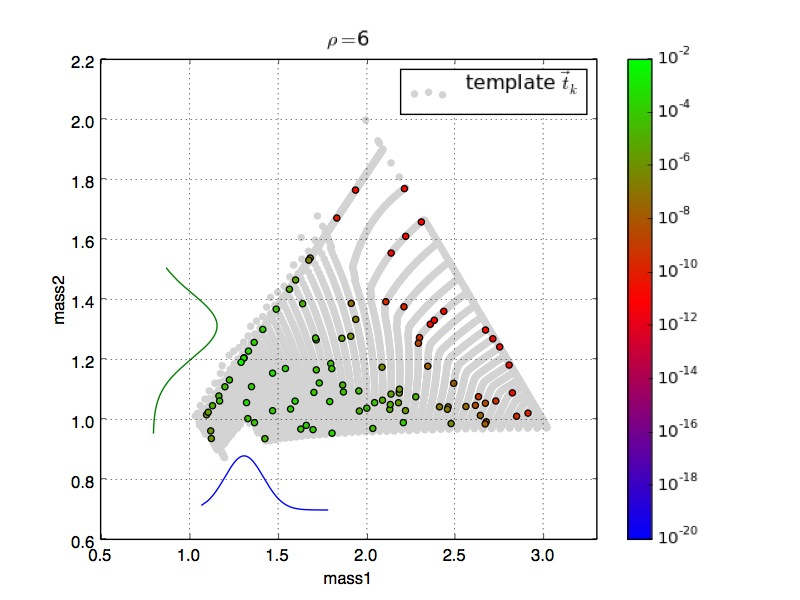
\includegraphics{first2years_20160612_P_tkj_100templates_6rho_N3.jpg}}
	\resizebox{\linewidth}{!}{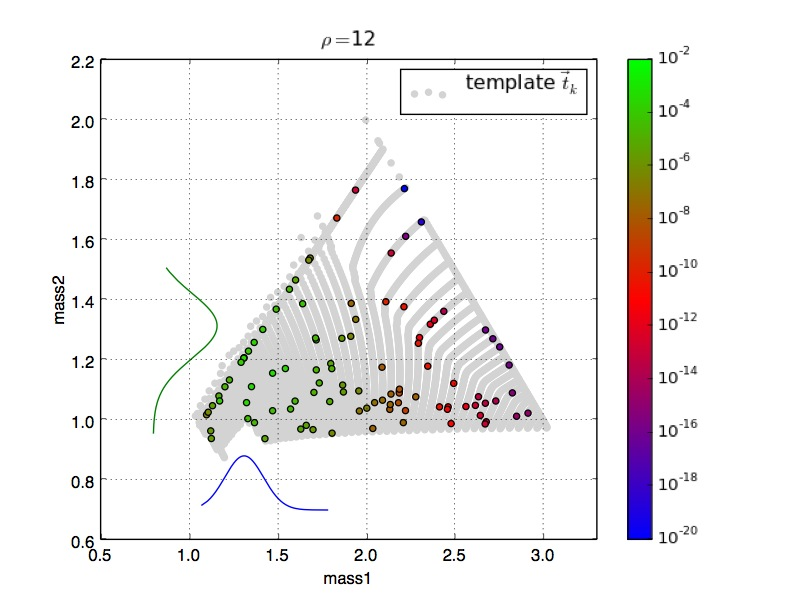
\includegraphics{first2years_20160612_P_tkj_100templates_12rho_N3.jpg}}
	\resizebox{\linewidth}{!}{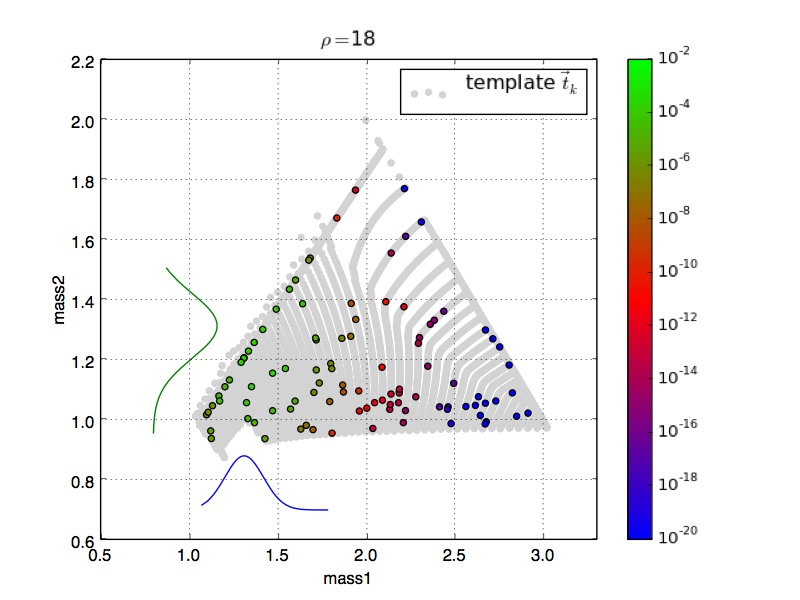
\includegraphics{first2years_20160612_P_tkj_100templates_18rho_N3.jpg}}
	\resizebox{\linewidth}{!}{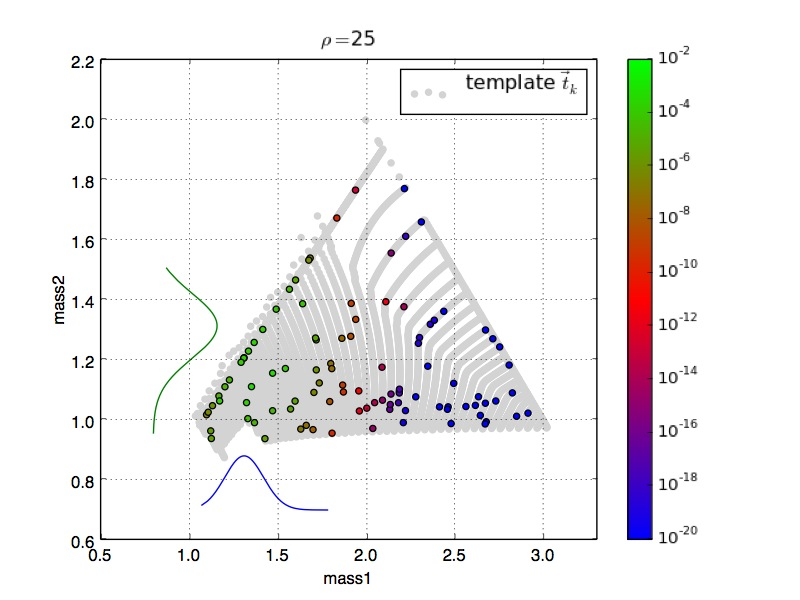
\includegraphics{first2years_20160612_P_tkj_100templates_25rho_N3.jpg}}
	\resizebox{\linewidth}{!}{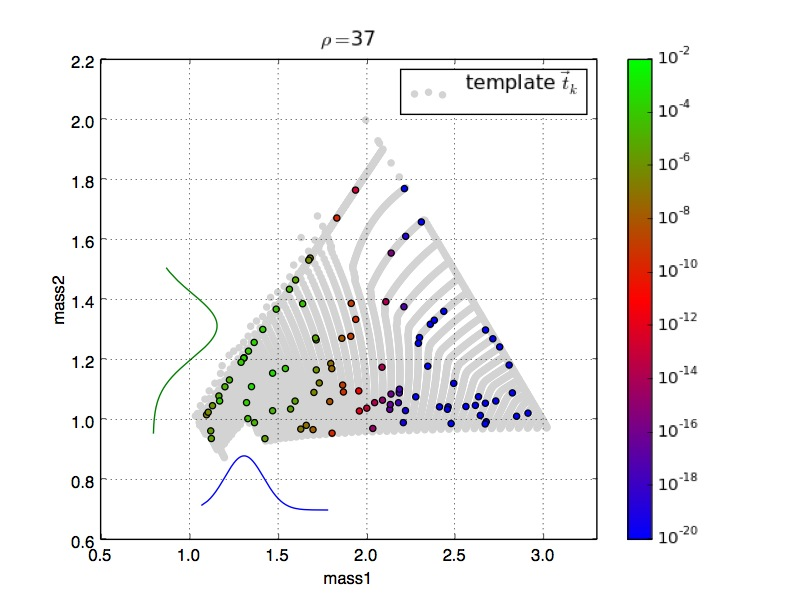
\includegraphics{first2years_20160612_P_tkj_100templates_37rho_N3.jpg}}
	\caption{100 templates were chosen at random, for which the probabilities $P(\text{all $\vec{s}$ in $\mathcal{S}$ is recoverable by $\vec{t}_k$})$ of each were calculated; the magnitude of the probability is given by the colour bar. The different plots show the probability calculated for different $\rho$. As $\rho$ is increased, the probability decreases for most templates, indicating that it is unlikely those templates will recover strong signals from our specified population. Some templates have probabilities that remain relatively constant with increasing $\rho$, and these tend to be clustered around the source population. While the colour scale only goes to $10^{-25}$, the probabilities at high $\rho$  go as low as $\sim\!10^{-52}$.}
	\label{fig:P_tkj}
	\end{figure}

%%%%%%%%%%%%%%%%%%%%%%%%%%
%%%%%%%%%%%%%%%%%%%%%%%%%%

\section{Conclusion}

\FIXME{Repeat reason as to why we need source-dependent ranking statistic, summarize that we derived the source dependency and implemented it into the ranking statistic. State results of the tests of estimating rates for two different source populations. Outline further work to be done. }

%%%%%%%%%%%%%%%%%%%%%%
\acknowledgments

Acknowledgements here


%%%%%%%%%%%%%%%%%%%%%%
\appendix

%%%%%%%%%%%%%%%%%%%%%%
\section{Distance and \ac{SNR}}
\label{appendix2}

Appendix goes here


%%%%%%%%%%%%%%%%%%%%%%
\bibliography{references}
\end{document}
